\chapter{Experiments \& Results} 
\label{chapter-experiments} 

In this chapter the attention module outlined in Chapter \ref{chapter-emma} will be evaluated in two main experiments. The first experiment evaluates the potential energy\footnote{Discussed Chapter \ref{chapter-energy-estimation}} as a differentiatior of failing modes on a real-case dataset. In the second experiment, the robustness and interpretability is analysed on an MMN, with and without EMMA.


%----------------------------------------------------------------------------------------
%	SECTION 
%----------------------------------------------------------------------------------------

\section{Pulsar Stars}
For the following experiments, our models will be trained on the HTRU2 dataset\footnote{The dataset can be found \href{https://archive.ics.uci.edu/ml/datasets/HTRU2}{here}, and was collected by \citep{HTRU}}, containing features describing radio emissions measured on Earth. The positive class corresponds to radio emissions of pulsars, which are a rare type of Neutron star that produce radio emission detectable here on Earth. They are of considerable scientific interest as probes of gravitational theories and time-keeping systems in spacecraft. A short summary of the seminal work of \citep{lyon} on this subject can be found in Appendix \ref{chapter-dataset}. 

The models will learn to distinguish pulsars from other radio emissions. The dataset consists of two modes:
\begin{itemize}
\item \textit{integrated profile} (IP): each pulsar produces a unique pattern of pulse emissions. The integrated profile is an average of these patterns over many thousands of rotations (further details in Appendix \ref{chapter-dataset}). The mode contains four features namely, the mean, standard deviation, excess kurtosis\footnote{Kurtosis refers to the size of the tails on a distribution. Excess kurtosis is a measure of how prone the distribution is to extreme outcomes.} and skewness of the integrated profile.
\item \textit{dispersion measure} (DM): the amount of dispersive smearing a signal receives is proportional to a quantity called the dispersion measure which is the integrated column density of free electrons between an observer and a pulsar (further details in Appendix \ref{chapter-dataset}). Similarly, the mode contains four features namely, the mean, standard deviation, excess kurtosis and skewness of the dispersion measure.
\end{itemize}

An additional difficulty of this dataset is that it is skewed, there are approximately ten time less positive samples than negative ones ($17.898$ total samples, $1.639$ positive samples, $16.259$ negative samples). This issue was handled by imposing a penalty in the loss function to fight the class imbalance.

In the experiments the dataset will be split into a training, validation and test set (see Table \ref{tab:split}). The validation set is used for tuning purposes, and to implement an Early Stopping\footnote{Early stopping \citep{early-stopping} is a form of regularization to avoid overfitting, where the error on the validation set is used in determining when overfitting has begun i.e., when the validation error starts increasing.} algorithm. Commonly, the model is then retrained for a few iterations on both the combined training and validation set, however, for the sake of simplicity, we do not retrain the models on the combined sets. Prior to the training, the data is standardized for the purpose of having the same signal-to-noise ratio corruption effect on all the features. To avoid information leakage, the statics (i.e., mean and variance) for the standardization are computed from the training set instead of the whole dataset, and applied to the three splits.
\begin{table}
\centering
\begin{tabular}{ r|cc|c } 
  & positive & negative & total \\ 
 \hline \hline
 train & 1.098 & 10.894 & 11.992 \\
 validation & 270 & 2.683 & 2.953 \\  
 test & 271 & 2.682 & 2.953 \\ 
 \hline
 total & 1.639 & 16.259 & 17.898 \\ 
 \hline
\end{tabular}
 \caption{Number of samples per split/class}
\label{tab:split}
\end{table}

%----------------------------------------------------------------------------------------
%	SECTION 
%----------------------------------------------------------------------------------------

\section{Experiment II}\label{sec:expII}
To verify whether the potential is a good measure of failure intensity, one autoencoder per mode was trained on the training set. Next, these autoencoders were evaluated on the test set, which partially contained noisy or out-of-distribution samples. The objective is to measure a clear difference in the values of the potential enery on the the failing samples. Notably, missing values are implicitly solved provided that they are replaced by zeros\footnote{$\beta\cdot 0 = 0,\,\forall \beta \in \mathbb{R}$}. With this in mind, we did not evaluate missing modes. Further details about the experimental setup are described in Appendix \ref{sec:setup-expII}.

\subsection*{Noisy values}
To simulate noisiness we add Gaussian white noise, $\mathcal{N} \sim (0,\sigma_{\text{corruption}}^2)$, to the test set. We compute the mean and variance of the potential energies of all the samples. This process is then repeated for different noise intensities. The result for each mode is show in Figure \ref{fig:pot-noisy-signal}. It is confirmed that potential energy can capture the noisiness of data, relative to the training samples.
\begin{figure}[!h]
\centering
\begin{subfigure}{.5\textwidth}
  \centering
  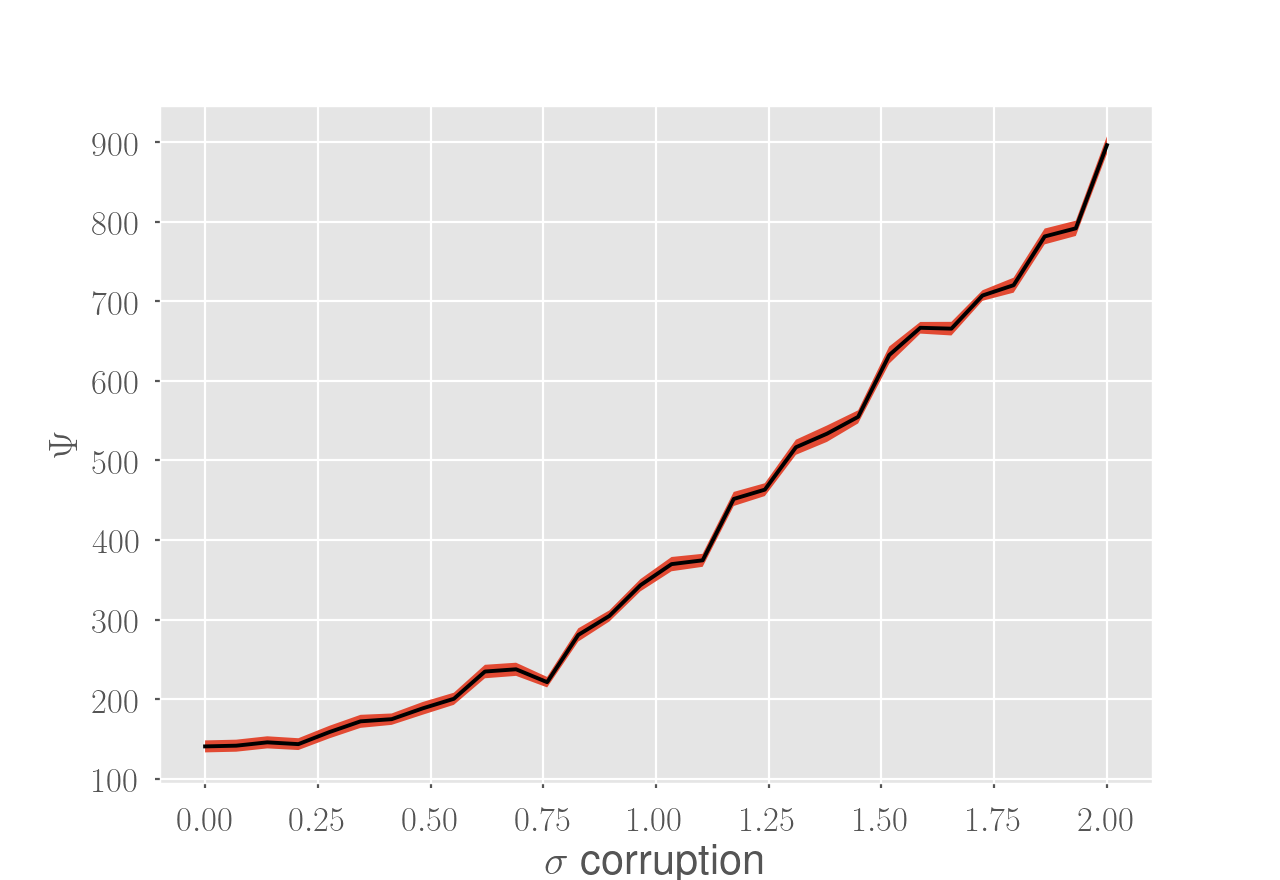
\includegraphics[width=\linewidth]{figures/noisy-signal-ip}
  \caption{IP mode}
\end{subfigure}%
\begin{subfigure}{.5\textwidth}
  \centering
  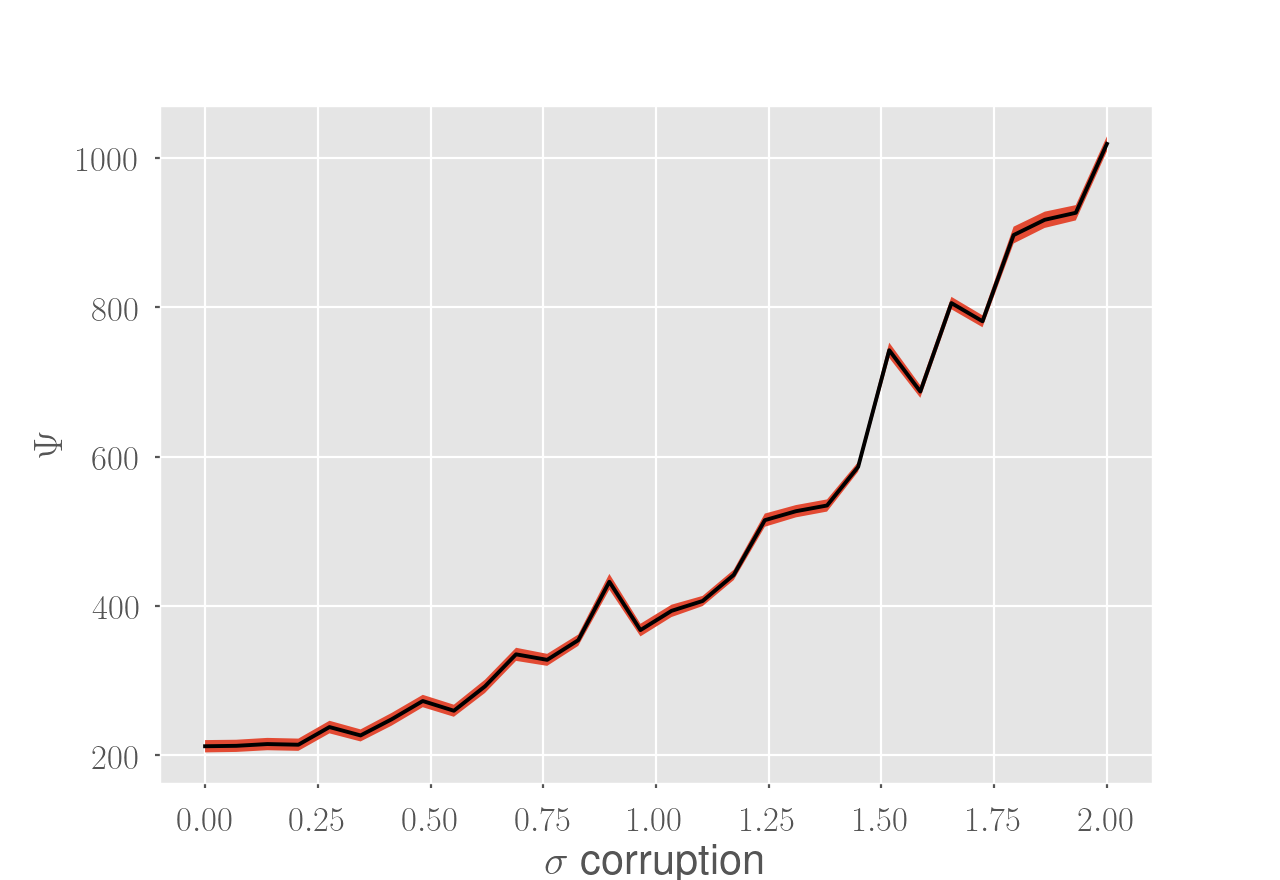
\includegraphics[width=\linewidth]{figures/noisy-signal-dm-snr}
  \caption{DM mode}
\end{subfigure}
\caption{Potential energy measured on noisy test samples (the mean corresponds to the black line, whereas the interval of two times the standard deviation error is displayed in red)}
\label{fig:pot-noisy-signal}
\end{figure}

\subsection*{Out-of-distribution samples}
Since we only have two classes, we modify the conventional procedure of training the autoencoders on all the samples, and instead train it only on positive samples. In this case, the negative samples can be considered as being out-of-distribution. The potential energies computed on the test set (containing positive and negative samples) were as expected (see Figure \ref{fig:pot-oof-signal}): potentials of likely data (positive) are lower and distinguishable from unlikely data (negative).
\begin{figure}[!h]
\centering
\begin{subfigure}{.5\textwidth}
  \centering
  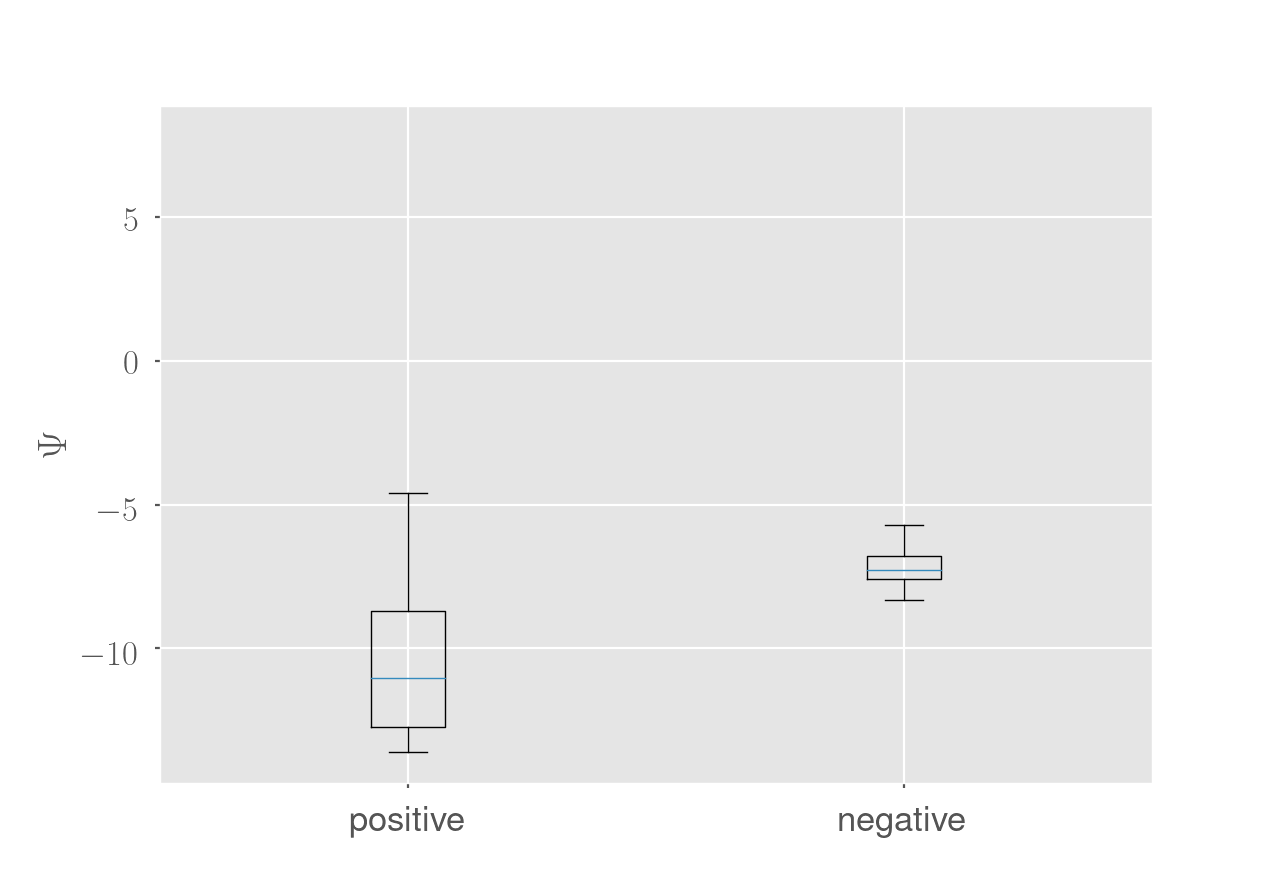
\includegraphics[width=\linewidth]{figures/signal-vs-background-ip}
   \caption{IP mode}
\end{subfigure}%
\begin{subfigure}{.5\textwidth}
  \centering
  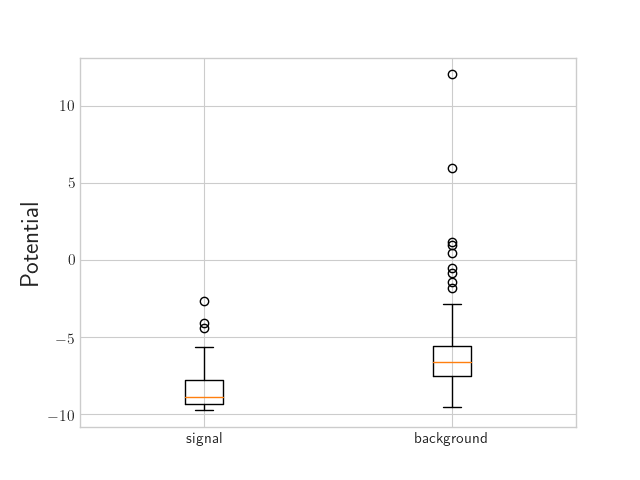
\includegraphics[width=\linewidth]{figures/signal-vs-background-dm-snr}
   \caption{DM mode}
\end{subfigure}
\caption{Potential energy measured on positive and negative samples, derived from autoencoders only trained on positive samples.}
\label{fig:pot-oof-signal}
\end{figure}


%----------------------------------------------------------------------------------------
%	SECTION 
%----------------------------------------------------------------------------------------

\newpage\section{Experiment III}\label{sec:expIII}
To asses the robustness gain from using EMMA along the MMN, we compare it with a standard data augmentation technique consisting in adding noisy samples to the training set in the hope that the MMN learns to suppress the noise by itself. Furthermore, three types of models will be evaluated:
\begin{itemize}
\item \texttt{base-model} is the MMN optimized on the training set (stage 1). Thus, without added noise neither using EMMA.
\item \texttt{model-without} is the model initialized with the weights of the \texttt{base-model}, and finetuned on a mix of corrupted and uncorrupted samples of the training set (data augmentation technique).
\item \texttt{model-with} is the combined \texttt{base-model} with the attention module EMMA. This model is trained end-to-end on a mix of corrupted and uncorrupted data (stage 2). Our hope is that the attention module will learn how to handle failing modes and be able to better generalize than  \texttt{model-without}. The MMN being released of this task, only has to learn to make predictions with available highlighted information.
\end{itemize}
The corruption process is applied in the following pattern: 50\% stays uncorrupted, 25\% noise on IP mode only, 25\% noise on DM mode only. The noisiness will be simulated by adding Gaussian white noise with a $\sigma_{\text{corruption}} = 0.5$.

The chosen loss function is the binary cross-entropy with an imbalance penalty. The three types of models are trained for 30 epochs with Early Stopping, where the variety implemented is as follows: at each epoch the state of the current model is saved as the new optimal one, if the validation  error is lower than the previous minima. Moreover, on the validation set the optimal classification threshold is determined by choosing the threshold on the ROC curve which is the nearest to the upper left corner.

In Table \ref{tab:results}, the F1-scores are showed of the three types of models on uncorrupted and corrupted samples\footnote{Same corruption process as the training set, $\sigma_{\text{corruption}} = 0.5$} of the test set. Several combinations (125) of hyperparameters were tested, only the fifteen best ones are displayed in the table below\footnote{Ranked by average F1-score on corrupted and uncorrupted samples}. Obviously, the \texttt{base-model} performs badly on samples with a noisy mode, since it was only trained on uncorrupted data. As can be seen, using data augmentation improves the performance on noisy data while being slightly worsened on uncorrupted samples. In contrast, models with our attention module outperform \texttt{model-without} and \texttt{base-model} by a significant margin. In the further experiment we will demonstrate how this difference is increased for more intensive failing modes. Surprisingly, some \texttt{model-with} slightly improve the F1-score on uncorrupted data of the \texttt{base-model}. No explanation could be found with certainty, however, it could be explained that EMMA is able to capture a certain spectrum of quality about the data, this information could then be used by the MMN to improve its predictions. Lastly, we can notice that the models are generally more robust when the failing mode is DM then when it is mode IP. This could mean that the IP mode carries more relevant information, since the SNR is the same on the two modes, we can rule out the possibility of a less sensitive mode.
\begin{table*}\centering
\ra{1.3}
\begin{tabular}{@{}rrrrcrrr@{}}\toprule
& \multicolumn{3}{c}{Hyperparameters} & \phantom{abc}& \multicolumn{3}{c}{F1-score}\\
\cmidrule{2-4} \cmidrule{6-8}
& \multicolumn{1}{c}{$\rho$} & \multicolumn{1}{c}{$\lambda_c$} & \multicolumn{1}{c}{$\lambda_e$} && \multicolumn{1}{r}{uncorrupted} & \multicolumn{1}{r}{IP noisy} & \multicolumn{1}{r}{DM noisy}\\ \midrule\midrule
base & & & && 0.8830 & 0.6441 & 0.6569\\
without & & & && 0.8671& 0.7097& 0.7683\\\midrule
with & $10^{-4}$ & $10^{-3}$ & $10^{-2}$ && $\mathbf{0.8881}$& $\mathbf{0.7333}$& $\mathbf{0.8077}$\\
with & $10^{-4}$ & $0$ & $10^{-2}$ && $\mathbf{0.8849}$& $\mathbf{0.7285}$& $\mathbf{0.8183}$\\
with & $10^{-4}$ & $10^{-4}$ & $10^{-2}$ && $\mathbf{0.8945}$& $\mathbf{0.7333}$& $\mathbf{0.8182}$\\
with & $10^{-3}$ & $10^{-3}$ & $0$ && 0.8809& $\mathbf{0.7347}$& $\mathbf{0.8186}$\\
with & $10^{-4}$ & $10^{-2}$ & $10^{-3}$ && 0.8736& $\mathbf{0.7383}$& $\mathbf{0.7848}$\\
with & $10^{-1}$ & $10^{-2}$ & $0$ && 0.8826& $\mathbf{0.7467}$& $\mathbf{0.7925}$\\
with & $10^{-4}$ & $10^{-3}$ & $0$ && 0.8786& $\mathbf{0.7190}$& $\mathbf{0.7826}$\\
with & $10^{-3}$ & $10^{-1}$ & $10^{-2}$ && 0.8800& $\mathbf{0.7432}$& $\mathbf{0.8344}$\\
with & $10^{-4}$ & $0$ & $10^{-4}$ && 0.8723& 0.7051& $\mathbf{0.7853}$\\
with & $10^{-4}$ & $10^{-4}$ & $10^{-3}$ && 0.8794& 0.7053& $\mathbf{0.7853}$\\
with & $10^{-3}$ & $10^{-3}$ & $10^{-4}$ && 0.8641& $\mathbf{0.7347}$& $\mathbf{0.8129}$\\
with & $1$ & $10^{-1}$ & $10^{-1}$ && 0.8683& $\mathbf{0.7237}$& $\mathbf{0.8052}$\\
with & $10^{-3}$ & $10^{-2}$ & $10^{-4}$ && 0.8705& $\mathbf{0.7105}$& $\mathbf{0.8205}$\\
with & $10^{-4}$ & $0$ & $10^{-3}$ && 0.8693& 0.7051& $\mathbf{0.7901}$\\
with & $10^{-3}$ & $10^{-1}$ & $0$ && 0.8817& 0.7049& $\mathbf{0.8129}$\\
\bottomrule
\end{tabular}
\caption{F1-scores of the top-15 trained models (the models are ranked by their weighted average F1-score)}
\label{tab:results}
\end{table*}

\subsection*{Attention-shift}
In order to study the attention shift, we display the importance and attention scores for different levels of noises. Figure \ref{fig:exp-att-shift-1} shows a clear attention shift. Interestingly, for a lower level of noise, more attention will be given to the IP-mode even when it is noisy, however, if the noise intensity is high enough the attention shifts towards the other mode (see Figure \ref{fig:exp-att-shift-1-d}). Notice that these results are consistent with Table \ref{tab:results} where we suggested that the IP mode seems to be more relevant. A more complete view of what the attention module actually learns is illustrated in Figure \ref{fig:mesh}.
\begin{figure}[!h]
\centering
\begin{subfigure}{.5\textwidth}
  \centering
  \includegraphics[width=\linewidth]{figures/noise-0-5/alpha-distrib-0}
  \caption{importance, noise $\sigma=0.5$} 
\end{subfigure}%
\begin{subfigure}{.5\textwidth}
  \centering
  \includegraphics[width=\linewidth]{figures/noise-0-5/beta-distrib-0}
  \caption{attention, noise $\sigma=0.5$} 
\end{subfigure}
\begin{subfigure}{.5\textwidth}
  \centering
  \includegraphics[width=\linewidth]{figures/noise-2/alpha-distrib-0}
  \caption{importance, noise $\sigma=2$} 
\end{subfigure}%
\begin{subfigure}{.5\textwidth}
  \centering
  \includegraphics[width=\linewidth]{figures/noise-2/beta-distrib-0}
  \caption{attention, noise $\sigma=2$} 
  \label{fig:exp-att-shift-1-d}
\end{subfigure}
\caption{Importance and attention scores for the $1^{\text{st}}$ ranked \texttt{model-with} ($\rho=10^{-4},\,\lambda_e=10^{-3},\,\lambda_c=10^{-2}$), on two different levels of noises}
\label{fig:exp-att-shift-1}
\end{figure}
\begin{figure}[!h]
\centering
\begin{subfigure}{.5\textwidth}
  \centering
  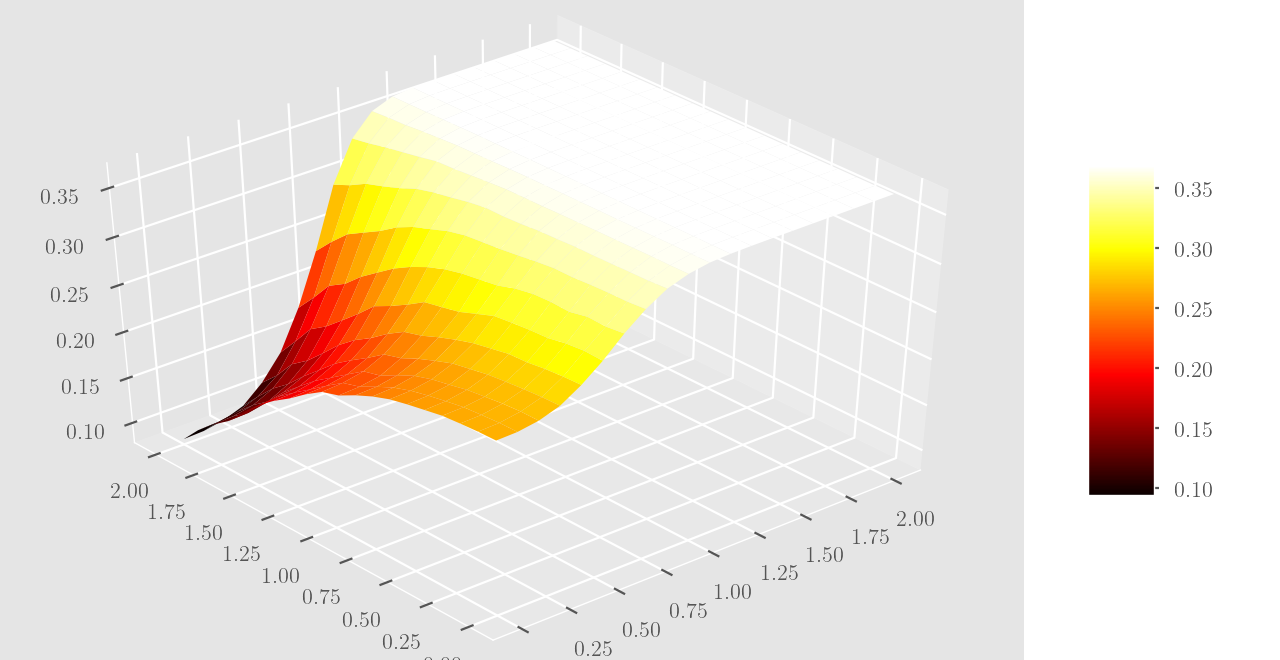
\includegraphics[width=\linewidth]{figures/Figure_1} 
  \caption{$\beta$-ip}
\end{subfigure}%
\begin{subfigure}{.5\textwidth}
  \centering
  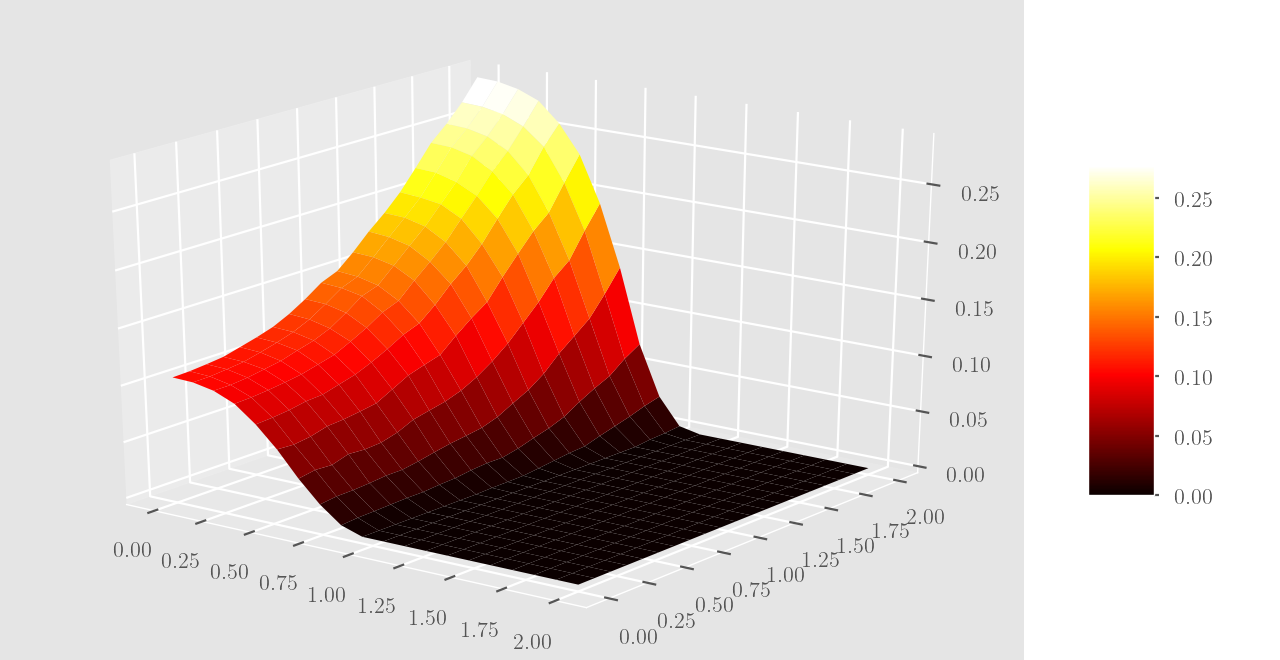
\includegraphics[width=\linewidth]{figures/Figure_2} 
  \caption{$\beta$-dm}
\end{subfigure}
\caption{3D visualization of attention scores on varying levels of noises between the modes (of the same model as Figure \ref{fig:exp-att-shift-1}}
\label{fig:mesh}
\end{figure}

In Figure \ref{fig:exp-att-shift-2}, the importance scores of two models trained with different temperatures are shown. As expected, the entropy of the importance scores is higher for the one with a low coldness $\rho$ (Figure \ref{fig:exp-att-shift-2-a}) enabling it to stay more stable for higher level of noise (Figure \ref{fig:exp-att-shift-2-b}). On the contrary, the model trained with a lower temperature has more pronounced attention shifts. To better visualise this, the attention scores are plotted on the continuum of noise intensities in Figure \ref{fig:exp-att-shift-3}. The crossing point in Figure \ref{fig:exp-att-shift-3-a} demonstrates that this model learns the trade-off between relevance and failure intensity. The model in Figure \ref{fig:exp-att-shift-3-c} is not able to learn it since its temperature and capacity are too high. Moreover, in Figure \ref{fig:exp-att-shift-4} it can be seen that regularizing the capacity too strongly can lead to a collapse of the attention scores i.e., all modes are masked.
\begin{figure}[!h]
\centering
\begin{subfigure}{.5\textwidth}
  \centering
  \includegraphics[width=\linewidth]{figures/noise-0-5/alpha-distrib-4}
  \caption{importance, $\rho=10^{-4}$, noise $\sigma=0.5$} 
  \label{fig:exp-att-shift-2-a}
\end{subfigure}%
\begin{subfigure}{.5\textwidth}
  \centering
  \includegraphics[width=\linewidth]{figures/noise-2/alpha-distrib-4}
  \caption{importance, $\rho=10^{-4}$, noise $\sigma=2$} 
  \label{fig:exp-att-shift-2-b}
\end{subfigure}
\begin{subfigure}{.5\textwidth}
  \centering
  \includegraphics[width=\linewidth]{figures/noise-0-5/alpha-distrib-5}
  \caption{importance, $\rho=10^{-1}$, noise $\sigma=0.5$} 
\end{subfigure}%
\begin{subfigure}{.5\textwidth}
  \centering
  \includegraphics[width=\linewidth]{figures/noise-2/alpha-distrib-5}
  \caption{importance, $\rho=10^{-1}$, noise $\sigma=2$} 
\end{subfigure}
\caption{Importance scores comparison of models with different temperatures: \texttt{model-with} ($\rho=10^{-4},\,\lambda_e=10^{-2},\,\lambda_c=10^{-3}$) and \texttt{model-with} ($\rho=10^{-1},\,\lambda_e=10^{-2},\,\lambda_c=0$)}
\label{fig:exp-att-shift-2}
\end{figure}

\begin{figure}[!h]
\centering
\begin{subfigure}{.5\textwidth}
  \centering
  \includegraphics[width=\linewidth]{figures/noise-generalisation-ip-noisy-beta-4}
  \caption{attention, $\rho=10^{-4}$, noise on IP} 
  \label{fig:exp-att-shift-3-a}
\end{subfigure}%
\begin{subfigure}{.5\textwidth}
  \centering
  \includegraphics[width=\linewidth]{figures/noise-generalisation-dm-noisy-beta-4}
  \caption{attention, $\rho=10^{-4}$, noise on DM} 
\end{subfigure}
\begin{subfigure}{.5\textwidth}
  \centering
  \includegraphics[width=\linewidth]{figures/noise-generalisation-ip-noisy-beta-5}
  \caption{attention, $\rho=10^{-1}$, noise on IP} 
  \label{fig:exp-att-shift-3-c}
\end{subfigure}%
\begin{subfigure}{.5\textwidth}
  \centering
  \includegraphics[width=\linewidth]{figures/noise-generalisation-dm-noisy-beta-5}
  \caption{attention, $\rho=10^{-1}$, noise on DM} 
\end{subfigure}
\caption{Attention scores comparison of models with different temperatures: \texttt{model-with} ($\rho=10^{-4},\,\lambda_e=10^{-2},\,\lambda_c=10^{-3}$) and \texttt{model-with} ($\rho=10^{-1},\,\lambda_e=10^{-2},\,\lambda_c=0$). The learned capacity for these models are respectively 0.49 and 0.63}
\label{fig:exp-att-shift-3}
\end{figure}

\begin{figure}[!h]
\centering
\begin{subfigure}{.5\textwidth}
  \centering
  \includegraphics[width=\linewidth]{figures/noise-0-5/alpha-distrib-103}
  \caption{Importance} 
\end{subfigure}%
\begin{subfigure}{.5\textwidth}
  \centering
  \includegraphics[width=\linewidth]{figures/noise-0-5/beta-distrib-103}
  \caption{Attention} 
\end{subfigure}
\caption{Importance and attention scores for \texttt{model-with} ($\rho=10^{-3},\,\lambda_e=10^{-4},\,\lambda_c=10^{-1}$). The learned capacity is 0.027}
\label{fig:exp-att-shift-4}
\end{figure}

\clearpage\subsection*{Total Energy}\label{sec:total-energy}
As mentionned previously, one of the advantages of the attention module is the interpretable clues it provides. One of those is the total energy, corresponding to the sum of all modal energies of the sample. To analyse this quantity, we add noise on both modes of the whole test set. Next, we compute the total energy and F1-score for each sample. This process is repeated for increasing noise intensity, as a result we show on Figure \ref{fig:exp-att-shift-5} the mean of the total energy and F1-score for each level of noise. A significant correlation can be observed between the two, hence, the total energy could be used as a proxy for uncertainty on the predictions. Remarkably, this pattern is observed in all the modules for whatever set of hyperparameters. The usefulness of the energy regularizer could thus be discused. However, in more complex datasets with more modes the coupling effect could cancel this correlation, in those cases the regularizer can help to find the optimal trade-off.
\begin{figure}[H]
\centering
\begin{subfigure}{.5\textwidth}
  \centering
  \includegraphics[width=\linewidth]{figures/noise-vs-system-energy}
\end{subfigure}%
\begin{subfigure}{.5\textwidth}
  \centering
  \includegraphics[width=\linewidth]{figures/noise-vs-system-f1}
\end{subfigure}
\caption{Total energy for \texttt{model-with} ($\rho=10^{-4},\,\lambda_e=10^{-3},\,\lambda_c=10^{-2}$)}
\label{fig:exp-att-shift-5}
\end{figure}

\subsection*{Robustness Generalisation}\label{sec:generalization}
As was discussed in Chapter \ref{chapter-literature-review}, robustness is often tested in the same conditions as the training. This does not seem to be a realistic assumption. To assess the robustness, we are going to check the F1-score on test set corrupted with varying levels of noises. What we would like to have is stability: it does not matter how high the perturbations are, if the other mode takes over the F1-score must keep stable. The $1^\text{st}$ ranked model in Table \ref{tab:results}, is evaluated in this manner and the results are shown in Figure \ref{fig:exp-att-shift-6}. When the DM mode is noisy (see Figure \ref{fig:exp-att-shift-6-b}), the module performs as we wish and masks the perturbations out thanks to EMMA which the other models are not able to do. There is still a small decrease in the F1-score of the attention module on the noisy DM mode, but this can be explained by the fact that we lose information form the DM-mode. For the IP-mode, the \texttt{model-with} does not perform better than \texttt{model-without} (Figure \ref{fig:exp-att-shift-6-a}). However, it can be observed that the performance seem to stabilize from the point the attention-shift between the mode occurs ($\sigma \approx 1.35$). To compare, we show another model (see Figure \ref{fig:exp-att-shift-7}) which learned a higher capacity (less regularization) and was thus able to learn the attention shift more optimally. As a consequence, we see that the F1-score remains drastically more constant (see Figure \ref{fig:exp-att-shift-7-a}). There is still a descrease, which is due to the loss of information of the IP-mode. Another example is shown in Figure \ref{fig:exp-att-shift-8}, were the the extreme case is shown for a too low capacity.
\begin{figure}[!h]
\centering
\begin{subfigure}{.5\textwidth}
  \centering
  \includegraphics[width=\linewidth]{figures/noise-generalisation-ip-noisy-0}
  \caption{F1-score, noisy IP-mode}
  \label{fig:exp-att-shift-6-a}
\end{subfigure}%
\begin{subfigure}{.5\textwidth}
  \centering
  \includegraphics[width=\linewidth]{figures/noise-generalisation-dm-noisy-0}
  \caption{F1-score, noisy DM-mode}
 \label{fig:exp-att-shift-6-b} 
\end{subfigure}
\begin{subfigure}{.5\textwidth}
  \centering
  \includegraphics[width=\linewidth]{figures/noise-generalisation-ip-noisy-beta-0}
  \caption{attention score, noisy IP-mode}
\end{subfigure}%
\begin{subfigure}{.5\textwidth}
  \centering
  \includegraphics[width=\linewidth]{figures/noise-generalisation-dm-noisy-beta-0}
  \caption{attention score, noisy DM-mode}
\end{subfigure}
\caption{Noise generalisation of \texttt{model-with} ($\rho=10^{-4},\,\lambda_e=10^{-3},\,\lambda_c=10^{-2}$). The learned capacity is 0.19}
\label{fig:exp-att-shift-6}
\end{figure}

\begin{figure}[!h]
\centering
\begin{subfigure}{.5\textwidth}
  \centering
  \includegraphics[width=\linewidth]{figures/noise-generalisation-ip-noisy-4}
  \caption{F1-score, noisy IP-mode}
  \label{fig:exp-att-shift-7-a}
\end{subfigure}%
\begin{subfigure}{.5\textwidth}
  \centering
  \includegraphics[width=\linewidth]{figures/noise-generalisation-dm-noisy-4}
  \caption{F1-score, noisy DM-mode}
\end{subfigure}
\begin{subfigure}{.5\textwidth}
  \centering
  \includegraphics[width=\linewidth]{figures/noise-generalisation-ip-noisy-beta-4}
  \caption{attention score, noisy IP-mode}
\end{subfigure}%
\begin{subfigure}{.5\textwidth}
  \centering
  \includegraphics[width=\linewidth]{figures/noise-generalisation-dm-noisy-beta-4}
  \caption{attention score, noisy DM-mode}
\end{subfigure}
\caption{Noise generalisation of \texttt{model-with} ($\rho=10^{-4},\,\lambda_e=10^{-2},\,\lambda_c=10^{-3}$). The learned capacity is 0.49}
\label{fig:exp-att-shift-7}
\end{figure}

\begin{figure}[!h]
\centering
\begin{subfigure}{.5\textwidth}
  \centering
  \includegraphics[width=\linewidth]{figures/noise-generalisation-ip-noisy-44}
  \caption{F1-score, noisy IP-mode}
\end{subfigure}%
\begin{subfigure}{.5\textwidth}
  \centering
  \includegraphics[width=\linewidth]{figures/noise-generalisation-dm-noisy-44}
  \caption{F1-score, noisy DM-mode}
\end{subfigure}
\begin{subfigure}{.5\textwidth}
  \centering
  \includegraphics[width=\linewidth]{figures/noise-generalisation-ip-noisy-beta-44}
  \caption{attention score, noisy IP-mode}
\end{subfigure}%
\begin{subfigure}{.5\textwidth}
  \centering
  \includegraphics[width=\linewidth]{figures/noise-generalisation-dm-noisy-beta-44}
  \caption{attention score, noisy DM-mode}
\end{subfigure}
\caption{Noise generalisation of \texttt{model-with} ($\rho=10^{-4},\,\lambda_e=10^{-1},\,\lambda_c=10^{-1}$). The learned capacity is 0.04}
\label{fig:exp-att-shift-8}
\end{figure}


\section{Limitation}
Several limitations of our experiments can be noticed:
\begin{itemize}
\item The main drawback is that the dataset only contained two modes, making it not possible to study asymmetric dependencies
\item The data were fairly simple. Not tested on high-dimensional complex data such as images. However, we think the module would perform even better since for such data suppressing noise is more difficult
\item Lastly no out-of-distribution class were in the dataset. As was shown in experiment II the potential energies seems able to distinguish it. The challenge would be to see if there is a conflict between the scales. Out-of-distribution samples with lower energies than noisy modes need to be more masked
\end{itemize}